\documentclass{article}

\usepackage{graphicx}
\usepackage{subfigure}

\begin{document}
	\listoffigures

	\subsection*{Ciudades Coloniales}

	\begin{figure}[!ht]
		\centering
		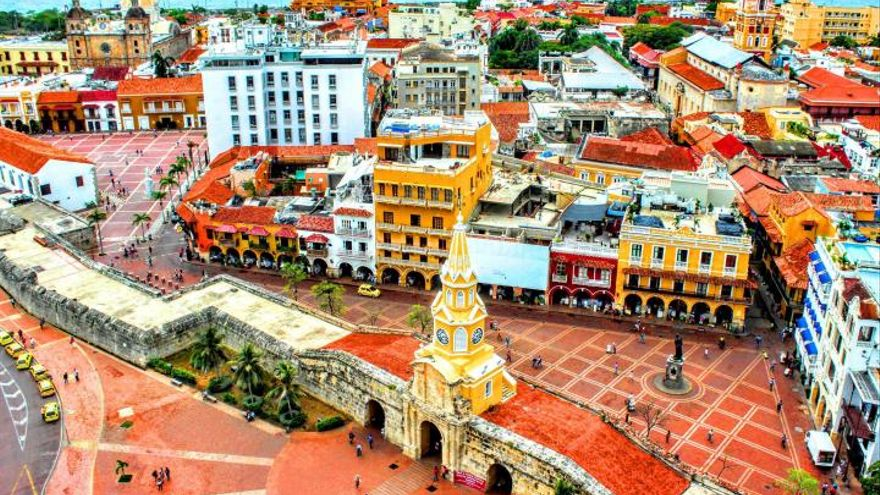
\includegraphics[width=8cm, height=6cm]{../images/cartagena_indias.jpg}
		\caption{Ciudad de Cartagena de Indias}
	\end{figure}

	\begin{figure}[!ht]
		\centering
		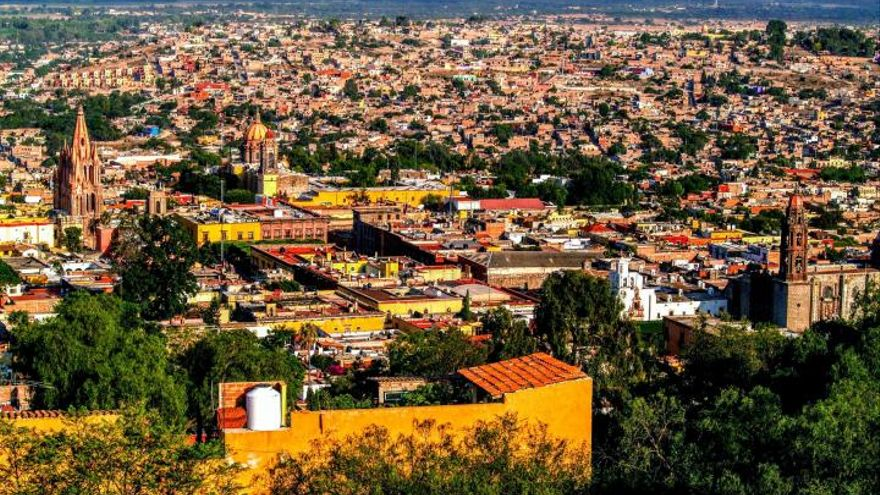
\includegraphics[width=8cm, height=6cm]{../images/san_miguel_allende.jpg}
		\caption{Ciudad de San Miguel Allende}
	\end{figure}

	\begin{figure}[!ht]
		\centering
		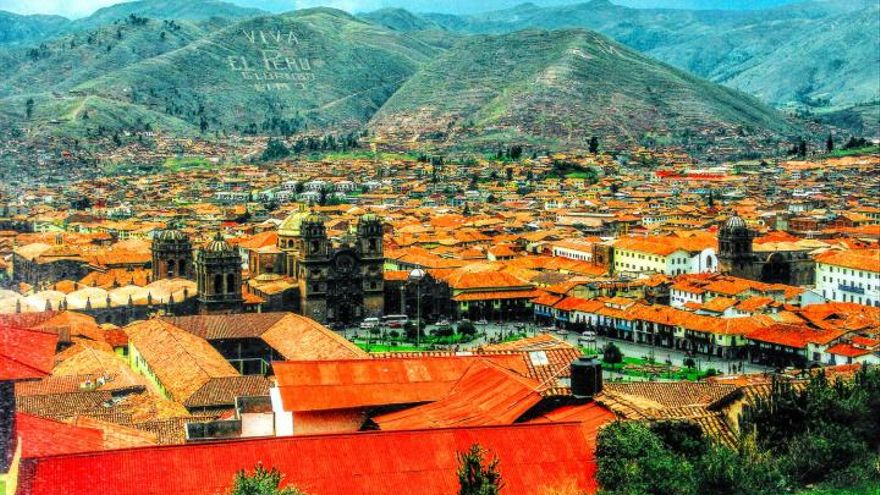
\includegraphics[width=10cm, height=7cm]{../images/cuzco.jpg}
		\caption{Ciudad de Cuzco}
	\end{figure}

	\subsection*{Figuras Planas}

	\begin{figure}[!ht]
		\centering
		\subfigure[Cuadrado]{
			
\includegraphics[width=2.5cm, height=2.5cm]{../images/figuras2d/cuadrado.png}
		}
		\subfigure[ Circulo]{
			
\includegraphics[width=2.5cm, height=2.5cm]{../images/figuras2d/circulo.png}
		}
		\subfigure[ Rombo]{
			
\includegraphics[scale=0.5]{../images/figuras2d/rombo.png}
		}
		\subfigure[ Pentagono]{
			
\includegraphics[scale=0.5, angle=45]{../images/figuras2d/pentagono.png}
		}
		\caption{Figuras geometricas de dos dimensiones}
	\end{figure}
\end{document}